%%%
\subsection{Combined fit results in unblinded SR}

We measure a signal strength parameter $\mu_{VBS} = 1.29 \pm 0.26$. Figure \ref{fig:postfitsr} shows the post-fit distributions for the 9 SRs with full range data while figure \ref{fig:postfitcr} shows the post-fit distributions for the 9 CRs of the analysis. These show quite good data to MC agreement.

\begin{figure}[h]
  \centering

  \subfigure[Resolved 0lep]{
    \includegraphics[width=.25\linewidth]{figures/StatisticalInterpretation/unblinded_postfit/Region_distRNN_DSRVBSTight_BMin0_T0_Y6051_incTag1_J2_L0_incJet1_GlobalFit_unconditionnal_mu1log}
  }
  \subfigure[Merged LP 0lep]{
    \includegraphics[width=.25\linewidth]{figures/StatisticalInterpretation/unblinded_postfit/Region_distRNN_DSRVBSLP_BMin0_J0_incJet1_L0_T0_incFat1_Y6051_incTag1_Fat1_GlobalFit_unconditionnal_mu1log}
  }
  \subfigure[Merged HP 0lep]{
    \includegraphics[width=.25\linewidth]{figures/StatisticalInterpretation/unblinded_postfit/Region_distRNN_DSRVBSHP_BMin0_J0_incJet1_L0_T0_incFat1_Y6051_incTag1_Fat1_GlobalFit_unconditionnal_mu1log}
  }

  \subfigure[Resolved 1lep]{
    \includegraphics[width=.25\linewidth]{figures/StatisticalInterpretation/unblinded_postfit/Region_distRNN_DSRVBSTight_BMin0_T0_Y6051_incTag1_J2_L1_incJet1_GlobalFit_unconditionnal_mu1log}
  }
  \subfigure[Merged LP 1lep]{
    \includegraphics[width=.25\linewidth]{figures/StatisticalInterpretation/unblinded_postfit/Region_distRNN_DSRVBSLP_BMin0_J0_incJet1_L1_T0_incFat1_Y6051_incTag1_Fat1_GlobalFit_unconditionnal_mu1log}
  }
  \subfigure[Merged HP 1lep]{
    \includegraphics[width=.25\linewidth]{figures/StatisticalInterpretation/unblinded_postfit/Region_distRNN_DSRVBSHP_BMin0_J0_incJet1_L1_T0_incFat1_Y6051_incTag1_Fat1_GlobalFit_unconditionnal_mu1log}
  }

    \subfigure[Resolved 2lep]{
    \includegraphics[width=.25\linewidth]{figures/StatisticalInterpretation/unblinded_postfit/Region_distRNN_DSRVBSTight_BMin0_T0_Y6051_incTag1_J2_L2_incJet1_GlobalFit_unconditionnal_mu1log}
  }
  \subfigure[Merged LP 2lep]{
    \includegraphics[width=.25\linewidth]{figures/StatisticalInterpretation/unblinded_postfit/Region_distRNN_DSRVBSLP_BMin0_J0_incJet1_L2_T0_incFat1_Y6051_incTag1_Fat1_GlobalFit_unconditionnal_mu1log}
  }
  \subfigure[Merged HP 2lep]{
    \includegraphics[width=.25\linewidth]{figures/StatisticalInterpretation/unblinded_postfit/Region_distRNN_DSRVBSHP_BMin0_J0_incJet1_L2_T0_incFat1_Y6051_incTag1_Fat1_GlobalFit_unconditionnal_mu1log}
  }

  \caption{Post-fit plots for SR distributions}
  \label{fig:postfitsr}
\end{figure}

\begin{figure}[h]
  \centering

  \subfigure[Resolved 0lep Vjet]{
    \includegraphics[width=.25\linewidth]{figures/StatisticalInterpretation/unblinded_postfit/Region_disttagMjj_DCRVjetTight_BMin0_T0_Y6051_incTag1_J2_L0_incJet1_GlobalFit_unconditionnal_mu1log}
  }
  \subfigure[Merged 0lep Vjet]{
    \includegraphics[width=.25\linewidth]{figures/StatisticalInterpretation/unblinded_postfit/Region_disttagMjj_DCRVjetMerged_BMin0_J0_incJet1_L0_T0_incFat1_Y6051_incTag1_Fat1_GlobalFit_unconditionnal_mu1log}
  }
  \subfigure[Resolved 1lep Top]{
    \includegraphics[width=.25\linewidth]{figures/StatisticalInterpretation/unblinded_postfit/Region_disttagMjj_DCRTopTight_BMin0_T0_Y6051_incTag1_J2_L1_incJet1_GlobalFit_unconditionnal_mu1log}
  }

  \subfigure[Resolved 1lep Vjet]{
    \includegraphics[width=.25\linewidth]{figures/StatisticalInterpretation/unblinded_postfit/Region_disttagMjj_DCRVjetTight_BMin0_T0_Y6051_incTag1_J2_L1_incJet1_GlobalFit_unconditionnal_mu1log}
  }
  \subfigure[Merged 1lep Vjet]{
    \includegraphics[width=.25\linewidth]{figures/StatisticalInterpretation/unblinded_postfit/Region_disttagMjj_DCRVjetMerged_BMin0_J0_incJet1_L1_T0_incFat1_Y6051_incTag1_Fat1_GlobalFit_unconditionnal_mu1log}
  }
  \subfigure[Merged LP 1lep Top]{
    \includegraphics[width=.25\linewidth]{figures/StatisticalInterpretation/unblinded_postfit/Region_disttagMjj_DCRTopLP_BMin0_J0_incJet1_L1_T0_incFat1_Y6051_incTag1_Fat1_GlobalFit_unconditionnal_mu1}
  }

  \subfigure[Resolved 2lep Vjet]{
    \includegraphics[width=.25\linewidth]{figures/StatisticalInterpretation/unblinded_postfit/Region_disttagMjj_DCRVjetTight_BMin0_T0_Y6051_incTag1_J2_L2_incJet1_GlobalFit_unconditionnal_mu1log}
  }
  \subfigure[Merged 2lep Vjet]{
    \includegraphics[width=.25\linewidth]{figures/StatisticalInterpretation/unblinded_postfit/Region_disttagMjj_DCRVjetMerged_BMin0_J0_incJet1_L2_T0_incFat1_Y6051_incTag1_Fat1_GlobalFit_unconditionnal_mu1log}
  }
  \subfigure[Merged HP 1lep Top]{
    \includegraphics[width=.25\linewidth]{figures/StatisticalInterpretation/unblinded_postfit/Region_disttagMjj_DCRTopHP_BMin0_J0_incJet1_L1_T0_incFat1_Y6051_incTag1_Fat1_GlobalFit_unconditionnal_mu1}
  }

  \caption{Post-fit plots for CR distributions}
  \label{fig:postfitcr}
\end{figure}

Tables \ref{tab:yields_unbl_srs}-\ref{tab:yields_unbl_crs} show post-fit event yields for all regions.

\begin{table}
\centering
\begin{tabular}{l|c|}
\hline
 & \multicolumn{1}{c|}{\zlep - SR Merged HP}\\
\hline
W & 557.68 $\pm$ 78.45\\
Z & 719.91 $\pm$ 96.67\\
Diboson & 316.82 $\pm$ 102.42\\
stop & 141.52 $\pm$ 37.83\\
ttbar & 1500.51 $\pm$ 131.22\\
\hline
Bkg & 3236.44 $\pm$ 59.70\\
\hline
EW6vvqq & 128.41 $\pm$ 23.50\\
\end{tabular}
\begin{tabular}{l|c|}
\hline
 & \multicolumn{1}{c|}{\olep - SR Merged HP}\\
\hline
W & 3148.88 $\pm$ 233.17\\
Z & 100.21 $\pm$ 47.84\\
Diboson & 919.44 $\pm$ 276.05\\
stop & 551.93 $\pm$ 148.00\\
ttbar & 7120.27 $\pm$ 261.57\\
\hline
Bkg & 11840.73 $\pm$ 110.42\\
\hline
EW6lvqq & 239.25 $\pm$ 49.70\\
\end{tabular}
\begin{tabular}{l|c|}
\hline
 & \multicolumn{1}{c|}{\tlep - SR Merged HP}\\
\hline
W & 0.39 $\pm$ 0.06\\
Z & 712.25 $\pm$ 48.41\\
Diboson & 169.08 $\pm$ 51.49\\
stop & 1.61 $\pm$ 0.63\\
ttbar & 27.90 $\pm$ 1.46\\
\hline
Bkg & 911.22 $\pm$ 26.48\\
\hline
EW6llqq & 49.14 $\pm$ 8.81\\
\end{tabular}
\begin{tabular}{l|c|}
\hline
 & \multicolumn{1}{c|}{\zlep - SR Merged LP}\\
\hline
W & 1616.36 $\pm$ 208.07\\
Z & 2240.60 $\pm$ 255.48\\
Diboson & 419.38 $\pm$ 135.22\\
stop & 180.09 $\pm$ 48.71\\
ttbar & 2027.05 $\pm$ 183.08\\
\hline
Bkg & 6483.50 $\pm$ 80.20\\
\hline
EW6vvqq & 93.83 $\pm$ 18.78\\
\end{tabular}
\begin{tabular}{l|c|}
\hline
 & \multicolumn{1}{c|}{\olep - SR Merged LP}\\
\hline
W & 9583.35 $\pm$ 484.77\\
Z & 289.32 $\pm$ 137.14\\
Diboson & 1281.29 $\pm$ 386.32\\
stop & 769.70 $\pm$ 209.67\\
ttbar & 10124.83 $\pm$ 458.76\\
\hline
Bkg & 22048.50 $\pm$ 179.56\\
\hline
EW6lvqq & 172.13 $\pm$ 43.02\\
\end{tabular}
\begin{tabular}{l|c|}
\hline
 & \multicolumn{1}{c|}{\tlep - SR Merged LP}\\
\hline
W & 1.29 $\pm$ 0.26\\
Z & 2174.74 $\pm$ 92.18\\
Diboson & 237.64 $\pm$ 72.95\\
stop & 3.00 $\pm$ 0.89\\
ttbar & 69.27 $\pm$ 4.21\\
\hline
Bkg & 2485.94 $\pm$ 44.10\\
\hline
EW6llqq & 37.33 $\pm$ 7.70\\
\end{tabular}
\begin{tabular}{l|c|}
\hline
 & \multicolumn{1}{c|}{\zlep - SR Resolved}\\
\hline
W & 8609.36 $\pm$ 790.07\\
Z & 10157.32 $\pm$ 867.25\\
Diboson & 609.81 $\pm$ 184.42\\
stop & 248.16 $\pm$ 66.46\\
ttbar & 1829.90 $\pm$ 242.39\\
\hline
Bkg & 21454.55 $\pm$ 152.18\\
\hline
EW6vvqq & 277.93 $\pm$ 56.14\\
\end{tabular}
\begin{tabular}{l|c|}
\hline
 & \multicolumn{1}{c|}{\olep - SR Resolved}\\
\hline
W & 58222.51 $\pm$ 895.83\\
Z & 1232.54 $\pm$ 545.70\\
Diboson & 1847.72 $\pm$ 524.97\\
stop & 1345.03 $\pm$ 358.58\\
ttbar & 7779.65 $\pm$ 329.45\\
\hline
Bkg & 70427.45 $\pm$ 350.90\\
\hline
EW6lvqq & 798.67 $\pm$ 178.56\\
\end{tabular}
\begin{tabular}{l|c|}
\hline
 & \multicolumn{1}{c|}{\tlep - SR Resolved}\\
\hline
W & 16.64 $\pm$ 2.16\\
Z & 25777.17 $\pm$ 249.07\\
Diboson & 627.18 $\pm$ 184.99\\
stop & 28.16 $\pm$ 7.89\\
ttbar & 875.13 $\pm$ 38.64\\
\hline
Bkg & 27324.27 $\pm$ 170.88\\
\hline
EW6llqq & 203.15 $\pm$ 43.19\\
\end{tabular}
\caption{Post-fit event yields for all the signal analysis regions.}
\label{tab:yields_unbl_srs}
\end{table}

\begin{table}
\centering  
\begin{tabular}{l|c|}
\hline
 & \multicolumn{1}{c|}{\olep - CR Top Merged HP}\\
\hline
W & 231.78 $\pm$ 17.19\\
Z & 10.62 $\pm$ 5.08\\
Diboson & 65.85 $\pm$ 20.06\\
stop & 1011.72 $\pm$ 269.07\\
ttbar & 10867.03 $\pm$ 296.53\\
\hline
Bkg & 12187.00 $\pm$ 107.78\\
\hline
EW6lvqq & 72.89 $\pm$ 19.80\\
\hline
data & 12195\\ \hline
\end{tabular}
\begin{tabular}{l|c|}
\hline
 & \multicolumn{1}{c|}{\olep - CR Top Merged LP}\\
\hline
W & 669.38 $\pm$ 37.40\\
Z & 30.73 $\pm$ 14.66\\
Diboson & 108.20 $\pm$ 32.51\\
stop & 1091.63 $\pm$ 299.56\\
ttbar & 15199.87 $\pm$ 397.39\\
\hline
Bkg & 17099.82 $\pm$ 185.02\\
\hline
EW6lvqq & 54.69 $\pm$ 14.82\\
\hline
data & 17195\\ \hline
\end{tabular}
\begin{tabular}{l|c|}
\hline
 & \multicolumn{1}{c|}{\olep - CR Top Resolved}\\
\hline
W & 2068.04 $\pm$ 85.96\\
Z & 66.18 $\pm$ 29.79\\
Diboson & 87.52 $\pm$ 24.90\\
stop & 1639.46 $\pm$ 437.33\\
ttbar & 12076.91 $\pm$ 474.27\\
\hline
Bkg & 15938.10 $\pm$ 132.64\\
\hline
EW6lvqq & 176.31 $\pm$ 40.63\\
\hline
data & 16131\\ \hline
\end{tabular}
\begin{tabular}{l|c|}
\hline
 & \multicolumn{1}{c|}{\zlep - CR Vjet Merged}\\
\hline
W & 4408.75 $\pm$ 581.28\\
Z & 6249.10 $\pm$ 715.86\\
Diboson & 853.81 $\pm$ 283.55\\
stop & 385.75 $\pm$ 105.03\\
ttbar & 4819.76 $\pm$ 600.96\\
\hline
Bkg & 16717.16 $\pm$ 144.40\\
\hline
EW6vvqq & 94.03 $\pm$ 20.41\\
\hline
data & 16833\\ \hline
\end{tabular}
\begin{tabular}{l|c|}
\hline
 & \multicolumn{1}{c|}{\olep - CR Vjet Merged}\\
\hline
W & 30124.87 $\pm$ 1817.94\\
Z & 922.58 $\pm$ 436.73\\
Diboson & 2804.42 $\pm$ 864.62\\
stop & 1987.11 $\pm$ 536.59\\
ttbar & 28040.44 $\pm$ 1585.06\\
\hline
Bkg & 63879.43 $\pm$ 274.69\\
\hline
EW6lvqq & 309.74 $\pm$ 99.39\\
\hline
data & 64166\\ \hline
\end{tabular}
\begin{tabular}{l|c|}
\hline
 & \multicolumn{1}{c|}{\tlep - CR Vjet Merged}\\
\hline
W & 2.48 $\pm$ 0.17\\
Z & 5913.81 $\pm$ 173.47\\
Diboson & 483.88 $\pm$ 152.81\\
stop & 6.37 $\pm$ 1.83\\
ttbar & 194.20 $\pm$ 10.46\\
\hline
Bkg & 6600.74 $\pm$ 82.69\\
\hline
EW6llqq & 40.21 $\pm$ 8.53\\
\hline
data & 6645\\ \hline
\end{tabular}
\begin{tabular}{l|c|}
\hline
 & \multicolumn{1}{c|}{\zlep - CR Vjet Resolved}\\
\hline
W & 64456.76 $\pm$ 5847.49\\
Z & 74216.66 $\pm$ 6529.95\\
Diboson & 4399.03 $\pm$ 1330.02\\
stop & 2625.80 $\pm$ 702.19\\
ttbar & 29626.24 $\pm$ 3593.24\\
\hline
Bkg & 175324.49 $\pm$ 492.92\\
\hline
EW6vvqq & 700.50 $\pm$ 121.87\\
\hline
data & 175982\\ \hline
\end{tabular}
\begin{tabular}{l|c|}
\hline
 & \multicolumn{1}{c|}{\olep - CR Vjet Resolved}\\
\hline
W & 502534.09 $\pm$ 10572.99\\
Z & 13911.50 $\pm$ 6100.56\\
Diboson & 15908.28 $\pm$ 4534.03\\
stop & 25533.03 $\pm$ 6859.05\\
ttbar & 228791.58 $\pm$ 10263.27\\
\hline
Bkg & 786678.48 $\pm$ 1628.97\\
\hline
EW6lvqq & 2257.53 $\pm$ 505.45\\
\hline
data & 788869\\ \hline
\end{tabular}
\begin{tabular}{l|c|}
\hline
 & \multicolumn{1}{c|}{\tlep - CR Vjet Resolved}\\
\hline
W & 72.17 $\pm$ 9.14\\
Z & 186850.95 $\pm$ 1501.30\\
Diboson & 4776.15 $\pm$ 1410.12\\
stop & 203.28 $\pm$ 55.23\\
ttbar & 7600.98 $\pm$ 435.29\\
\hline
Bkg & 199503.53 $\pm$ 480.59\\
\hline
EW6llqq & 534.59 $\pm$ 102.13\\
\hline
data & 200097\\ \hline
\end{tabular}
\caption{Post-fit event yields for all the control analysis regions.}
\label{tab:yields_unbl_crs}
\end{table}

Table \ref{fig:break} shows the uncertainty breakdown on $\mu_{VBS}$.

\begin{table}[h]
  \centering
  \includegraphics[width=0.5\textwidth]{figures/StatisticalInterpretation/unblinded_postfit/new_breakdown}
  \caption{Uncertainty breakdown on $\mu_{VBS}$ in combined fit.}
  \label{tab:break}
\end{table}

Figure \ref{fig:corr} shows the correlation matrix for full range data fit.

\begin{figure}[h]
  \centering
  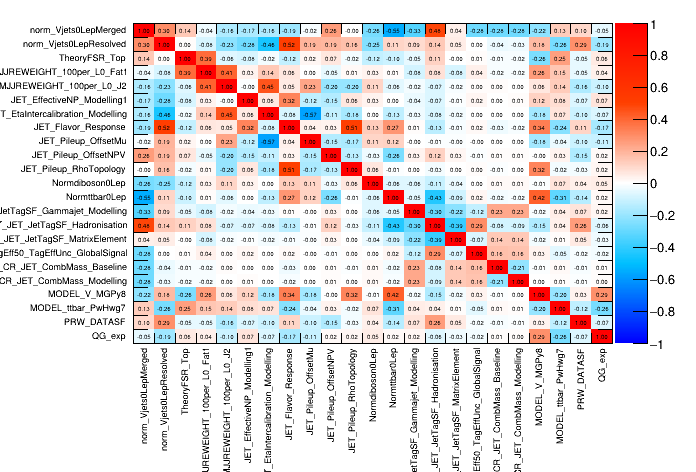
\includegraphics[width=0.9\textwidth]{figures/StatisticalInterpretation/unblinded_postfit/corr_HighCorrNoMCStat}
  \caption{Correlations in full SR data range fit.}
  \label{fig:corr}
\end{figure}

Figure \ref{fig:rankCombine} shows the ranking plots for the combined full range data fit. The most leading uncertainties impacting the fitted $\mu$ are the Theory QCD and shower uncertainty on the signal, the re-weighting in the \tlep channel, the modeling uncertainty of the \Zjets background in the \tlep channel and the \Wjets background in the \olep channel and the EW-QCD interference uncertainty in the \olep channel.

\begin{figure}[h]
  \centering
  \subfigure[Prefit combined]{\includegraphics[width=0.49\textwidth]{figures/StatisticalInterpretation/new_rankings/Ranking_prefit_mu_SemileptonicVBS}}
  \subfigure[Postfit combined]{\includegraphics[width=0.49\textwidth]{figures/StatisticalInterpretation/new_rankings/Ranking_postfit_mu_SemileptonicVBS}}
  \caption{Ranking of nuisance parameters prefit-sorted and postfit-sorted for the combined fit.}
  \label{fig:rankCombine}
\end{figure}

%%%
\subsection{Single lepton channels results}

Figure \ref{fig:singlepostfitsr} shows the post-fit distributions for the SRs for single lepton channels full range fits and figure \ref{fig:singlepostfitcr} shows the post-fit distributions for the CRs.

\begin{figure}[h]
  \centering

  \subfigure[Resolved 0lep]{
    \includegraphics[width=.25\linewidth]{figures/0lep/unblinded_postfit/Region_distRNN_DSRVBSTight_BMin0_T0_Y6051_incTag1_J2_L0_incJet1_GlobalFit_unconditionnal_mu1log}
  }
  \subfigure[Merged LP 0lep]{
    \includegraphics[width=.25\linewidth]{figures/0lep/unblinded_postfit/Region_distRNN_DSRVBSLP_BMin0_J0_incJet1_L0_T0_incFat1_Y6051_incTag1_Fat1_GlobalFit_unconditionnal_mu1log}
  }
  \subfigure[Merged HP 0lep]{
    \includegraphics[width=.25\linewidth]{figures/0lep/unblinded_postfit/Region_distRNN_DSRVBSHP_BMin0_J0_incJet1_L0_T0_incFat1_Y6051_incTag1_Fat1_GlobalFit_unconditionnal_mu1log}
  }

  \subfigure[Resolved 1lep]{
    \includegraphics[width=.25\linewidth]{figures/1lep/unblinded_postfit/Region_distRNN_DSRVBSTight_BMin0_T0_Y6051_incTag1_J2_L1_incJet1_GlobalFit_unconditionnal_mu1log}
  }
  \subfigure[Merged LP 1lep]{
    \includegraphics[width=.25\linewidth]{figures/1lep/unblinded_postfit/Region_distRNN_DSRVBSLP_BMin0_J0_incJet1_L1_T0_incFat1_Y6051_incTag1_Fat1_GlobalFit_unconditionnal_mu1log}
  }
  \subfigure[Merged HP 1lep]{
    \includegraphics[width=.25\linewidth]{figures/1lep/unblinded_postfit/Region_distRNN_DSRVBSHP_BMin0_J0_incJet1_L1_T0_incFat1_Y6051_incTag1_Fat1_GlobalFit_unconditionnal_mu1log}
  }

    \subfigure[Resolved 2lep]{
    \includegraphics[width=.25\linewidth]{figures/2lep/unblinded_postfit/Region_distRNN_DSRVBSTight_BMin0_T0_Y6051_incTag1_J2_L2_incJet1_GlobalFit_unconditionnal_mu1log}
  }
  \subfigure[Merged LP 2lep]{
    \includegraphics[width=.25\linewidth]{figures/2lep/unblinded_postfit/Region_distRNN_DSRVBSLP_BMin0_J0_incJet1_L2_T0_incFat1_Y6051_incTag1_Fat1_GlobalFit_unconditionnal_mu1log}
  }
  \subfigure[Merged HP 2lep]{
    \includegraphics[width=.25\linewidth]{figures/2lep/unblinded_postfit/Region_distRNN_DSRVBSHP_BMin0_J0_incJet1_L2_T0_incFat1_Y6051_incTag1_Fat1_GlobalFit_unconditionnal_mu1log}
  }

  \caption{Single channel post-fit plots for SR distributions}
  \label{fig:singlepostfitsr}
\end{figure}

\begin{figure}[h]
  \centering

  \subfigure[Resolved 0lep Vjet]{
    \includegraphics[width=.25\linewidth]{figures/0lep/unblinded_postfit/Region_disttagMjj_DCRVjetTight_BMin0_T0_Y6051_incTag1_J2_L0_incJet1_GlobalFit_unconditionnal_mu1log}
  }
  \subfigure[Merged 0lep Vjet]{
    \includegraphics[width=.25\linewidth]{figures/0lep/unblinded_postfit/Region_disttagMjj_DCRVjetMerged_BMin0_J0_incJet1_L0_T0_incFat1_Y6051_incTag1_Fat1_GlobalFit_unconditionnal_mu1log}
  }
  \subfigure[Resolved 1lep Top]{
    \includegraphics[width=.25\linewidth]{figures/1lep/unblinded_postfit/Region_disttagMjj_DCRTopTight_BMin0_T0_Y6051_incTag1_J2_L1_incJet1_GlobalFit_unconditionnal_mu1log}
  }

  \subfigure[Resolved 1lep Vjet]{
    \includegraphics[width=.25\linewidth]{figures/1lep/unblinded_postfit/Region_disttagMjj_DCRVjetTight_BMin0_T0_Y6051_incTag1_J2_L1_incJet1_GlobalFit_unconditionnal_mu1log}
  }
  \subfigure[Merged 1lep Vjet]{
    \includegraphics[width=.25\linewidth]{figures/1lep/unblinded_postfit/Region_disttagMjj_DCRVjetMerged_BMin0_J0_incJet1_L1_T0_incFat1_Y6051_incTag1_Fat1_GlobalFit_unconditionnal_mu1log}
  }
  \subfigure[Merged LP 1lep Top]{
    \includegraphics[width=.25\linewidth]{figures/1lep/unblinded_postfit/Region_disttagMjj_DCRTopLP_BMin0_J0_incJet1_L1_T0_incFat1_Y6051_incTag1_Fat1_GlobalFit_unconditionnal_mu1}
  }

  \subfigure[Resolved 2lep Vjet]{
    \includegraphics[width=.25\linewidth]{figures/2lep/unblinded_postfit/Region_disttagMjj_DCRVjetTight_BMin0_T0_Y6051_incTag1_J2_L2_incJet1_GlobalFit_unconditionnal_mu1log}
  }
  \subfigure[Merged 2lep Vjet]{
    \includegraphics[width=.25\linewidth]{figures/2lep/unblinded_postfit/Region_disttagMjj_DCRVjetMerged_BMin0_J0_incJet1_L2_T0_incFat1_Y6051_incTag1_Fat1_GlobalFit_unconditionnal_mu1log}
  }
  \subfigure[Merged HP 1lep Top]{
    \includegraphics[width=.25\linewidth]{figures/1lep/unblinded_postfit/Region_disttagMjj_DCRTopHP_BMin0_J0_incJet1_L1_T0_incFat1_Y6051_incTag1_Fat1_GlobalFit_unconditionnal_mu1}
  }

  \caption{Single channel post-fit plots for CR distributions}
  \label{fig:singlepostfitcr}
\end{figure}

Table \ref{tab:significance} shows the expected and observed significances for single channels as well as for the combined fit. The observed significance is greater than 5$\sigma$ in the combined channel.

\begin{table}[h]
  \centering
  \begin{tabular}{|c|c|c|c|c|}
    \hline
           & 0-lep & 1-lep & 2-lep & combined \\
    \hline
    Expected pre-fit significance & 3.00 & 4.80 & 2.52 & 6.15 \\
    \hline
    Expected post-fit significance & 2.96 & 4.47 & 2.64 & 5.96 \\
    \hline
    Observed significance & 5.53 & 4.03 & 3.08 & 7.30 \\
    \hline
  \end{tabular}
  \caption{Expected and observed significances for the single channel and combined fit.}
  \label{tab:significance}
\end{table}

We observe an important excess compared to the expected significance in the \zlep channel and some deficit in the \olep channel.

%%%
\subsection{Multi-POIs fits}

For multi-POI fits, the summary of the significance is reported in Table \ref{tab:significance2} and the summary of the fitted POI is reported in Figure \ref{fig:fit:sigStrenghtCombine}.

\begin{table}[h]
  \centering
  \begin{tabular}{|c|c|c|c|c|}
    \hline
     & 0-lep & 1-lep & 2-lep & combined \\
    \hline
    Decorr 3POI & 6.40 & 4.59 & 2.88 & | \\
    \hline
    Decorr 6POI & 5.27 & 5.00 & 1.23 & Resolved \\
    Decorr 6POI & 4.09 & 1.18 & 3.36 & Merged \\
    \hline
    Decorr 2POI & | & | & Resolved & 6.52 \\
    Decorr 2POI & | & | & Merged   & 3.77 \\
    \hline
    Decorr 2POI & | & | & VBS & 6.18 \\
    Decorr 2POI & | & | & VV  & 3.89 \\
    \hline
    Decorr 4POI & | & | & VBS Resolved & 5.42 \\
    Decorr 4POI & | & | & VBS Merged & 3.36 \\
    Decorr 4POI & | & | & VV Resolved & 0.98 \\
    Decorr 4POI & | & | & VV Merged & 3.85 \\
    \hline
  \end{tabular}
  \caption{Observed significance for different POI fit configurations.}
  \label{tab:significance2}
\end{table}

\begin{figure}[h]
  \centering
  \includegraphics[width=.8\textwidth]{figures/StatisticalInterpretation/unblinded_postfit/Muhat_VBS_channels_all}
  \caption{Signal strength parameter from different fits.}
  \label{fig:fit:sigStrenghtCombine}
\end{figure}

$\mu_{VBS}$ doesn't vary considerably when floating $\mu_{QCDVV}$. The compatibility between 1 and 3 POI fits is 3.4\% while the compatibility between 1 and 2 POI (Resolved/Merged) fits is 28.4\% and the compatibility between 1 and 6 POI fits is 0.42\%. In addition the compatibility between 2 (VBS/VV) and 4 POI fits is 37.4\%. We can see in Figure \ref{fig:corr2POI} that the correlation between the two POIs is -25\%.

\begin{figure}[h]
  \centering
  \includegraphics[width=0.9\textwidth]{figures/StatisticalInterpretation/unblinded_postfit/corr_HighCorrNoMCStat2POI}
  \caption{Correlations for the fit floating both VBS and VV background.}
  \label{fig:corr2POI}
\end{figure}

The 2D contour plot for $\mu_{VBS}$ vs $\mu_{QCDVV}$ can be found in Figure \ref{fig:contour}. The measurements are $2\sigma$ away from the SM.

\begin{figure}[h]
  \centering
  \includegraphics[width=0.6\textwidth]{figures/StatisticalInterpretation/unblinded_postfit/contours}
  \caption{2D contour floating $\mu_{VBS}$ and $\mu_{QCDVV}$ in unblinded fit.}
\label{fig:contour}
\end{figure}




